\chapter{Descripción del Trabajo}
\label{cap:descripcionTrabajo}

Aquí comienza la descripción del trabajo realizado. Se deben incluir tantos capítulos como sea necesario para describir de la manera más completa posible el trabajo que se ha llevado a cabo. Como muestra la figura \ref{fig:sampleImage}, está todo por hacer.

\begin{figure}[h]
	\centering
	
\includegraphics[width = 0.5\textwidth]{Imagenes/Vectorial/Todo.pdf}
	\caption{Ejemplo de imagen}
	\label{fig:sampleImage}
\end{figure}

Si te sirve de utilidad,  puedes incluir tablas para mostrar resultados, tal como se ve en la tabla \ref{tab:sampleTable}.


\begin{table}
	\centering
	\begin{tabular}{c|c|c}
		\textbf{Col 1} & \textbf{Col 2} & \textbf{Col 3} \\
		\hline\hline
		3 & 3.01 & 3.50\\
		6 & 2.12 & 4.40\\
		1 & 3.79 & 5.00\\
		2 & 4.88 & 5.30\\
		4 & 3.50 & 2.90\\
		5 & 7.40 & 4.70\\
		\hline
	\end{tabular}
	\caption{Tabla de ejemplo}
	\label{tab:sampleTable}
\end{table}

\section{Funcionamiento de una OCR}
El OCR (Reconocimiento Óptico de Caracteres, por sus siglas en inglés Optical Character Recognition) es una tecnología que convierte imágenes de texto manuscrito, impreso o mecanografiado en datos de texto que las computadoras pueden interpretar y manipular , en otras palabras , puede extraer el texto contenida en una imagen.

Para llegar al objetivo de reconocer el texto y extraerlo de la imagen el ocr da una serie de pasos:
\begin{enumerate}
	\item \textbf{Preprocesamiento de la imagen:}
	
	El propósito de este paso es procesar la imagen para que sea más legible para la computadora ,reconocer así de forma mas eficiente los textos.
	\begin{itemize}
		\item Conversión a escala de grises: La mayoría de los OCR primero convierten la imagen en blanco y negro o escala de grises para simplificar el procesamiento.
		\item Reducción de ruido: Se aplican filtros para eliminar manchas, borrones o marcas en la imagen que puedan afectar la precisión del reconocimiento.
		\item Binarización: La imagen se convierte a una representación en blanco y negro, donde los píxeles se clasifican como parte del fondo (blanco) o del texto (negro). Este proceso ayuda a aislar los caracteres.
	\end{itemize}
	
	\item \textbf{Segmentación:}
	
	 El OCR divide la imagen en secciones manejables, primero separa líneas de texto, luego separa las palabras y finalmente descompone las palabras en caracteres individuales.Este paso es crucial, ya que el OCR necesita reconocer los caracteres de manera individual, pero considerando también su contexto dentro de una palabra o frase.
	
	\item \textbf{Detección de características:}
	
	Extracción de características de los caracteres: El OCR analiza los caracteres y sus formas, midiendo varios atributos como las líneas, contornos, cruces de líneas, y la disposición de los píxeles. Estos datos son usados para diferenciar letras, números y símbolos similares (como ``O'' y ``0'' o ``l'' y ``1'').
	Se aplican técnicas basadas en modelos geométricos, estructuras de redes neuronales o de aprendizaje automático para identificar patrones comunes en los caracteres.
	
	\item \textbf{Reconocimiento del carácter:}
	
	Clasificación de los caracteres: Una vez identificadas las características, el OCR las compara con una base de datos o ``alfabeto'' interno de posibles caracteres. Esto puede hacerse de varias maneras, dependiendo del tipo de OCR:
	\begin{itemize}
		\item Métodos basados en plantillas: Se compara cada carácter con un conjunto de plantillas predefinidas. Si la forma del carácter coincide con una plantilla, se clasifica como ese carácter.
		\item Métodos basados en aprendizaje automático o redes neuronales: Las técnicas modernas de OCR suelen usar redes neuronales entrenadas con miles de ejemplos de texto. El sistema "aprende" a identificar caracteres y a hacer distinciones más sutiles en base a sus experiencias pasadas.
	\end{itemize}
		\item \textbf{Post-procesamiento:}
	
	\begin{itemize}
		\item Corrección de errores: Una vez que el OCR ha reconocido los caracteres, puede haber errores, especialmente si el texto es borroso o está en una fuente inusual. Por lo tanto, muchos OCR incluyen un corrector ortográfico o usan diccionarios para identificar palabras que no tienen sentido y corregirlas basándose en el contexto.
		\item Reconstrucción del formato: Algunos OCR también intentan mantener el formato original del documento, incluyendo aspectos como la disposición de las columnas, el tipo de letra, negritas, subrayados, etc.
		
	\end{itemize}
		\item \textbf{Conversión a texto:}
		
		Una vez que se han identificado todos los caracteres, el OCR genera una salida de texto editable, que se puede guardar en un archivo o ser exportado a otros formatos como PDF o documento de Word.
	
		
\end{enumerate}
	
\section{Selección de OCR (Optical Character Recognition)}
Durante el desarrollo de este trabajo, se evaluaron varias herramientas de Reconocimiento Óptico de Caracteres (OCR) para seleccionar la más adecuada para nuestras necesidades. Las herramientas probadas fueron Ocropus, EasyOCR y Tesseract. A continuación, se describe brevemente cada una de ellas, seguida de las razones por las cuales se eligió Tesseract para el proyecto.Las pruebas de las ocr se realizan con la misma imagen:
\begin{figure}[h]
	\centering
	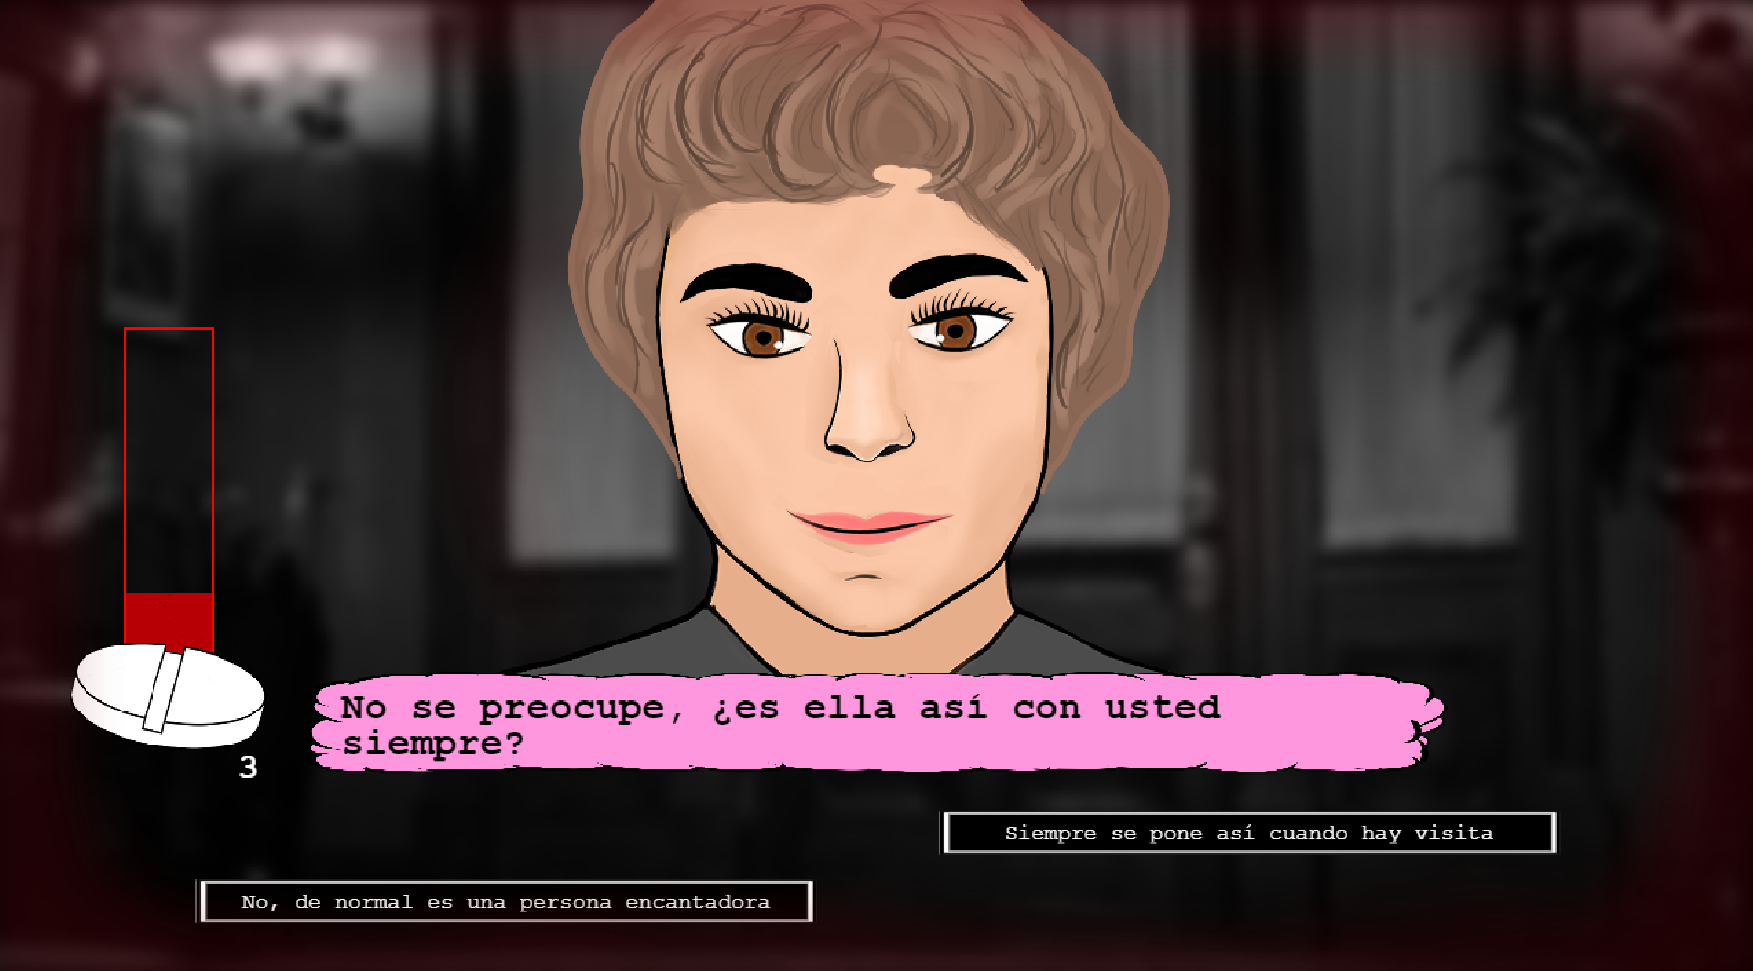
\includegraphics[width = 0.5\textwidth]{Imagenes/OCR/GameScene.png}
	\caption{Imagen de prueba para los OCR}
\end{figure}
\begin{enumerate}
	\item \textbf{Ocropus}
	
	Es un sistema de OCR basado en redes neuronales con un enfoque modular.
	Principalmente esta disponible para linux , proporciona diferentes módulos para la binarización , segmentación ,generación del ground-truth y el entreno del modelo.
	Se ha utilizado la herramienta para reconocer la imagen de prueba pero el resultado fue que no consiguió reconocer ningún texto , por lo que fue descartado ya que las otras alternativas que hablaremos en adelante si que ha conseguido algo.
	Otras razones por la que esta herramienta fue descartado es que el lenguaje de programación principal con la que trabaja es \emph{python} y en nuestro proyecto trabajamos principalmente con \emph{c++} , además la última actualización de esta librería fue en 16 de Diciembre de 2017\footnote{\url{https://github.com/ocropus-archive/DUP-ocropy} (repositorio github de Ocropus)}
	
	\item \textbf{EasyOCR}
	
	EasyOCR es una biblioteca de reconocimiento óptico de caracteres (OCR) desarrollada en Python que facilita la extracción de texto de imágenes y documentos. Diseñada con el objetivo de ser fácil de usar y accesible, una de las características de EasyOCR es que es capaz de reconocer texto en más de 80 idiomas y soporta múltiples scripts, lo que la convierte en una herramienta versátil para diversas aplicaciones.
	La herramienta es fácil de usar (no tienes que hacer tu todo el proceso de binarización , segmentación,...) y ofrece buenos resultados al reconocimiento.
	Proporciona gran variedad de modelos entrenados y también ofrece la opción de entrenar tu propio modelo.
	Se ha realizado la misma prueba de la imagen con esta herramienta (figura \ref{fig:EasyOCR_Test}) , en este caso para facilitar el proceso , se ha utilizado directamente la página demo que proporciona EasyOCR\footnote{\url{https://www.jaided.ai/easyocr/} (Demo de EasyOCR)}
	
	\begin{figure}[h]
			\centering
			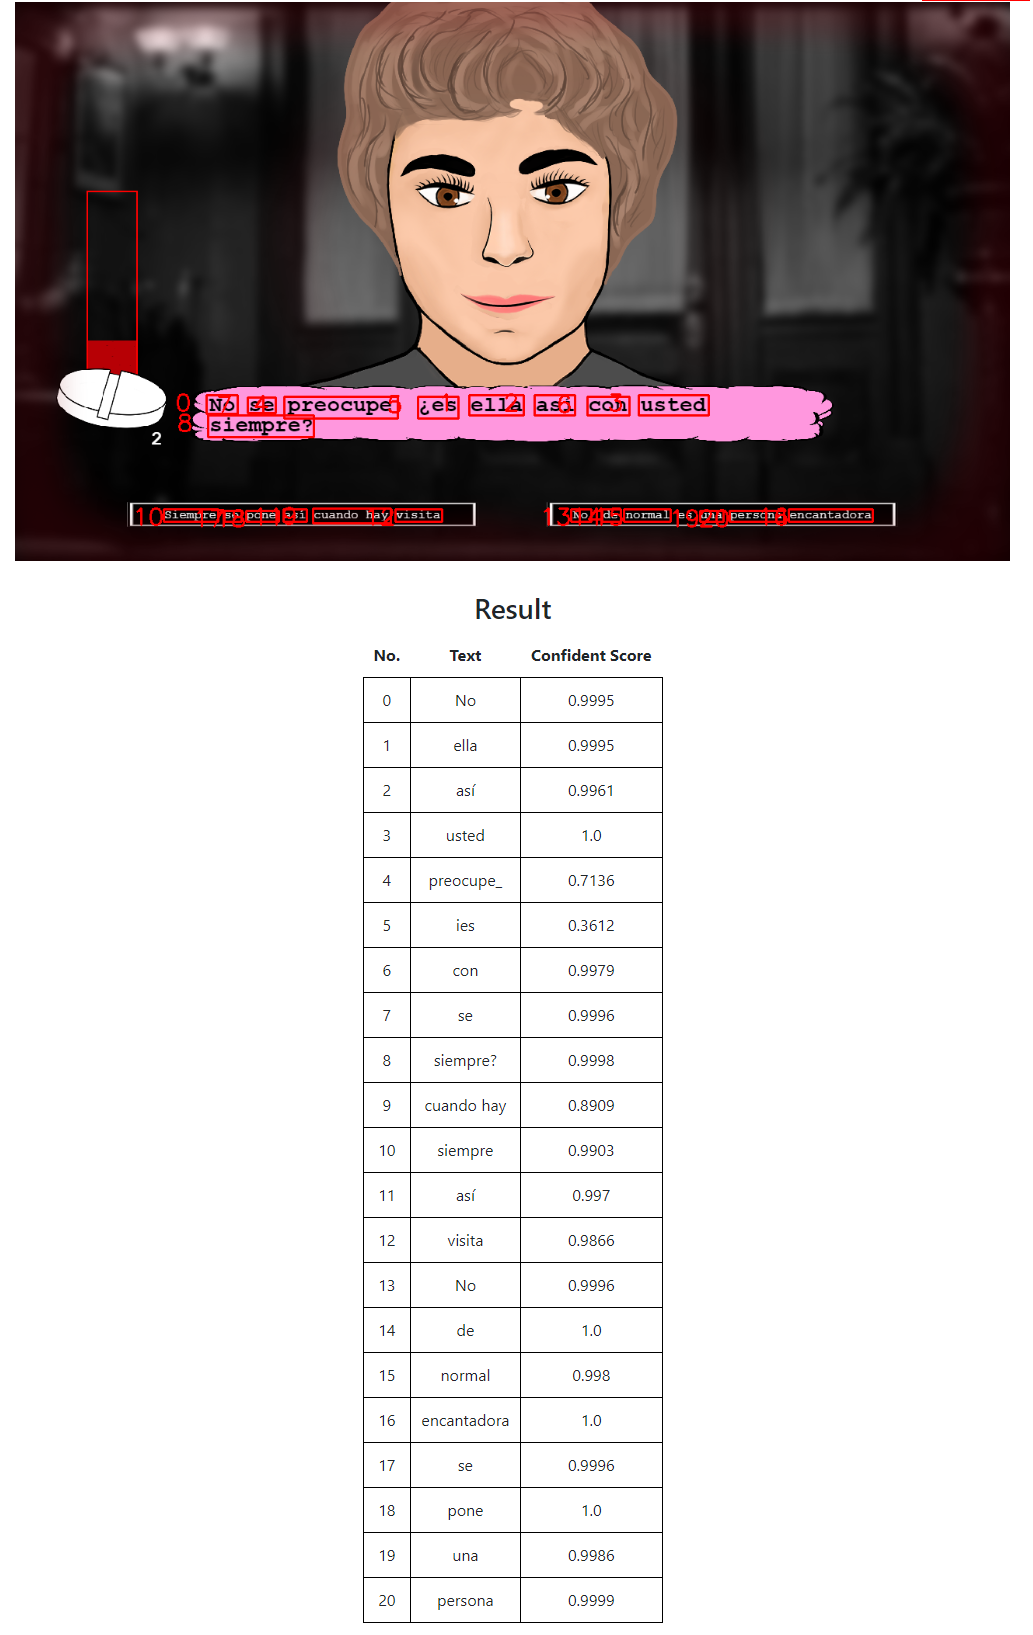
\includegraphics[width = 0.5\textwidth]{Imagenes/OCR/EasyOcr_Test.png}
			\caption{Resultado de EasyOCR}
			\label{fig:EasyOCR_Test}
	\end{figure}
	La herramienta en resumen se adapta muy bien a nuestras necesidades , el único problema esta en el idioma de programación con la que trabaja , al igual que ocropus , EasyOCR trabaja principalmente con \emph{python} y nosotros con \emph{c++} , esto no supone un gran problema pero hemos encontrado una mejor solución , Tesseract.
	
	\item \textbf{Tesseract}
	Tesseract es un motor de reconocimiento óptico de caracteres (OCR) de código abierto que se utiliza para convertir imágenes de texto en texto editable. Originalmente desarrollado por Hewlett-Packard en la década de 1980, Tesseract fue liberado como software de código abierto en 2005 y ha sido mantenido y mejorado por la comunidad, particularmente por Google, que ha contribuido significativamente a su desarrollo.
	
	Al igual que EasyOCR una de las características más destacadas de Tesseract es su capacidad para reconocer texto en múltiples idiomas y alfabetos, soportando más de 100 idiomas de forma nativa. Esto lo convierte en una herramienta versátil para aplicaciones globales que requieren la extracción de texto de documentos escritos en diferentes lenguas.
	
	Tesseract utiliza técnicas avanzadas de aprendizaje profundo y redes neuronales, lo que le permite alcanzar altos niveles de precisión en el reconocimiento de texto. Su arquitectura se basa en el uso de modelos de aprendizaje profundo entrenados con grandes conjuntos de datos, lo que mejora continuamente su rendimiento en diversas condiciones.
	
	El motor puede integrarse fácilmente en aplicaciones de procesamiento de imágenes y visión por computadora. Tesseract se utiliza comúnmente en combinación con bibliotecas como OpenCV para preprocesar imágenes antes de la etapa de reconocimiento, lo que mejora la precisión de los resultados.
	
	Además, Tesseract ofrece una API en varios lenguajes de programación, lo que facilita su integración en diferentes entornos de desarrollo y una de ellas es C++ , por lo que esta herramienta cumple con todos los requisitos para nuestro proyecto y es la razón por la que hemos optado por Tesseract.
\end{enumerate}
\section{Descripción de los tests}
\subsection{Testing sobre errores de cadena no localizada - detección de placeholder}
\begin{itemize}
	\item Problema: \\
	Sucede cuando el texto incluye placeholders de variables p.ej \{name\}  \\
	\item Entrada: \\
	Cadena leída por el detector de texto \\
	Marcadores de placeholder \\
	\item Comportamiento: \\
	El test asume que los marcadores de placeholder no se usan de manera natural en el lenguaje escrito.
	Lo que hará el test es leer la string de entrada y contar el número de caracteres hasta que aparezca un marcador de inicio de placeholder. En ese momento se guardará el número de caracteres hasta esa primera aparición, y después guardará la string que aparece de ese momento hasta que se encuentre un marcador de cierre de placeholder. 
	Al final, el test escribirá en pantalla el número del carácter en el que empieza cada placeholder y la cadena de texto que haya dentro de dicho placeholder.
\end{itemize}

\subsection{Testing sobre problema de fuente
}
\begin{itemize}
	\item Problema: \\
	La fuente utilizada no incluye alguno de los caracteres especiales de un idioma , por ejemplo las tildes (á) , la ñ en español.  \\
	\item Entrada: \\
	Cadena leída por el detector de texto
	
	Cadena de texto esperado
	
	\item Comportamiento: \\
	El test leerá la cadena de texto leída por el detector y las compara uno a uno con la cadena de texto esperado , se guardará la posición en la que son distintos y se mostrará en la salida el número de caracteres distintos y su posición.
	
\end{itemize}



\subsection{Testing sobre cadena de texto no localizada}
\begin{itemize}
	\item Problema: \\

	\item Entrada: \\

	\item Comportamiento: \\

\end{itemize}
\subsection{Testing sobre solapamiento de texto}

\begin{itemize}
	\item Problema: \\
	Cuando el texto escrito es más largo de lo esperado por el programador por lo que se sale de los límites del espacio guardado para ese texto y se solapan. \\
	\item Entrada: \\
	
	\item Comportamiento: \\
	
\end{itemize}
\subsection{Testing sobre truncamiento de texto
}
\begin{itemize}
	\item Problema: \\
	
	\item Entrada: \\
	
	\item Comportamiento: \\
	
\end{itemize}
\subsection{Testing sobre error tipográfico/gramatical
}
\begin{itemize}
	\item Problema: \\
	
	\item Entrada: \\
	
	\item Comportamiento: \\
	
\end{itemize}
 

